\section{World Models}
\label{sec:world_models}
\label{sec:architectures}
\label{sec:training}

\begin{figure*}[t]
\centering
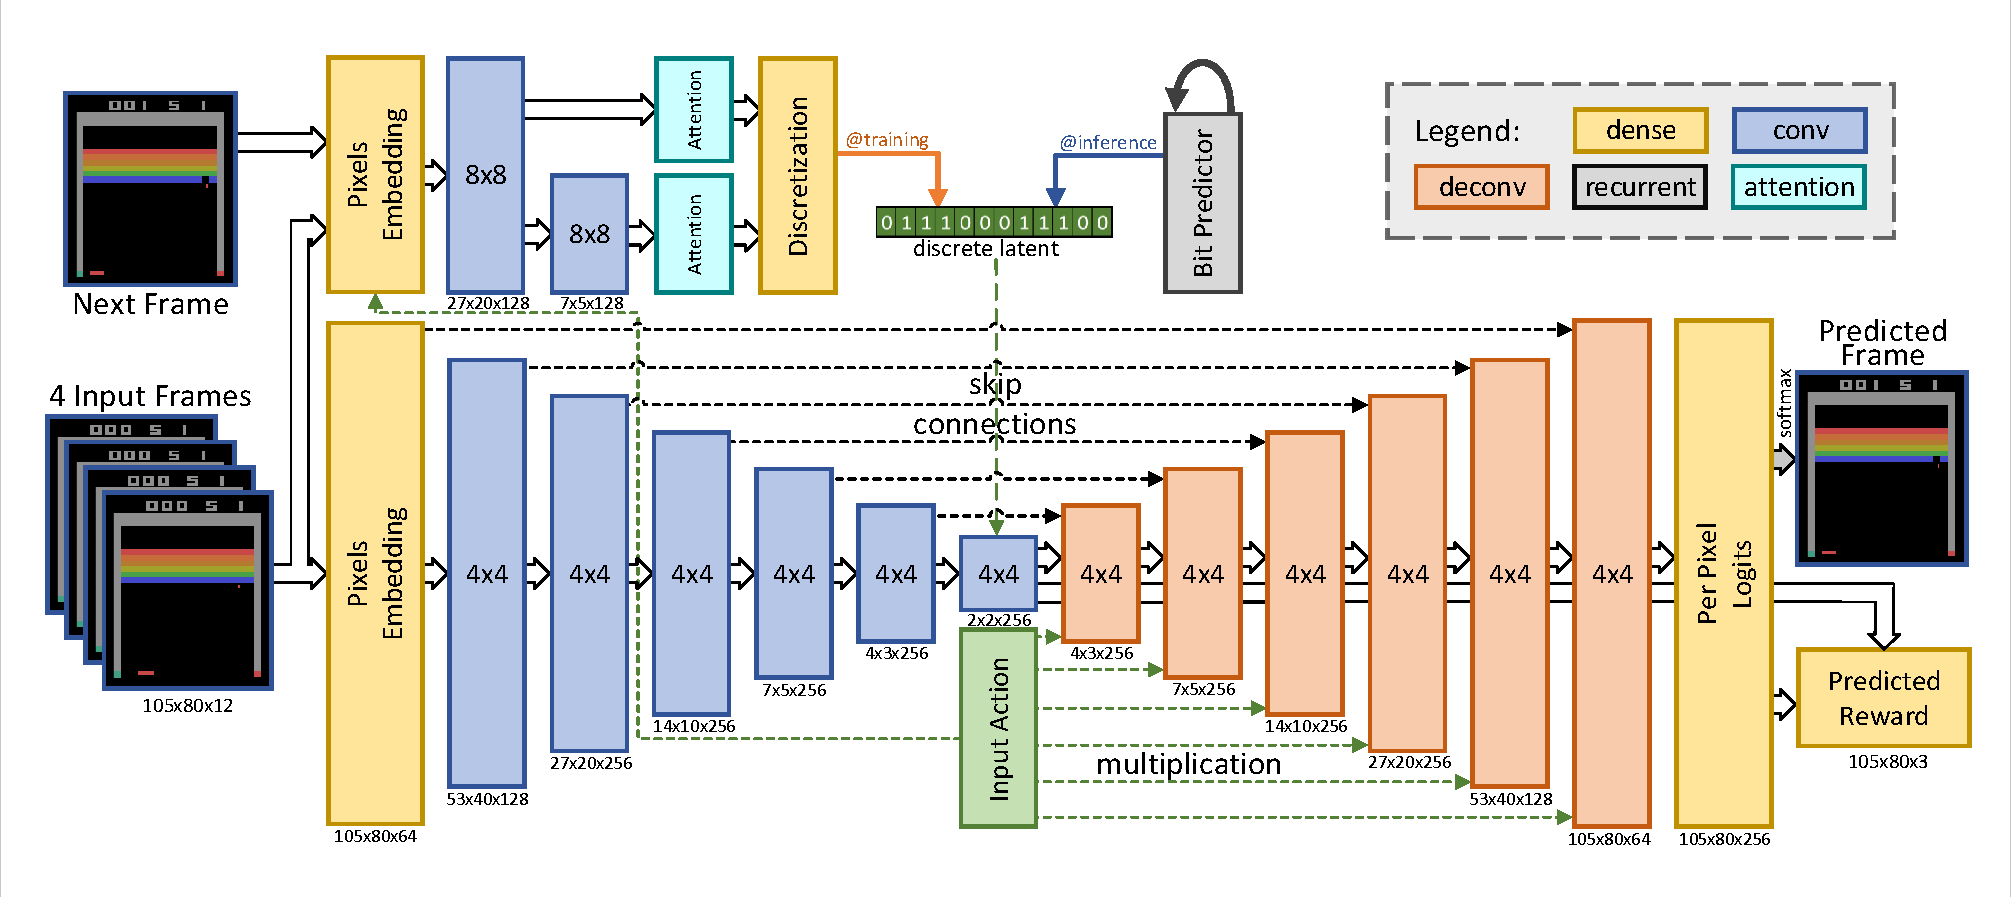
\includegraphics[width=1.0\textwidth]{figures/model_basic_disc.pdf}
\caption{Architecture of the proposed stochastic model with discrete latent. The input to the model is four stacked frames (as well as the action selected by the agent) while the output is the next predicted frame and expected reward. Input pixels and action are embedded using fully connected layers, and there is per-pixel softmax ($256$ colors) in the output. This model has two main components. First, the bottom part of the network which consists of a skip-connected convolutional encoder and decoder. To condition the output on the actions of the agent, the output of each layer in the decoder is multiplied with the (learned) embedded action. Second part of the model is a convolutional inference network which approximates the posterior given the next frame similar to~\citet{sv2p}. At training time, the sampled latent values from the approximated posterior will be discretized into bits. To keep the model differentiable, the backpropagation bypasses the discretization following~\citet{auto_discrete}. A third LSTM based network is trained to approximate each bit given the previous ones. At inference time, the latent bits are predicted auto-regressively using this network. The deterministic model has the same architecture as this figure but without the inference network.}
\label{fig:full_discrete}
\end{figure*}




A crucial decision in the design of world models   %
is the inclusion of stochasticity. Although Atari is known to be a deterministic environment, it is stochastic given only a limited horizon of past observed frames (in our case $4$ frames). The level of stochasticity is game dependent; however, it can be observed in many Atari games. An example of such behavior is the \textit{pause} after a player scores in \texttt{Pong}. These pauses are longer than 4 frames, so a model looking at only the past 4 frames does not know when a new round of the game should start and may keep predicting paused frames.

In search for an effective world model we have experimented with various architectures, both new and modified versions of existing ones. In this section, we describe the architectures and the rationale behind our design decisions.  In Section \ref{sec:analysis} we compare the performance of these models.

\subsection{Deterministic Model}
Our basic architecture, presented as part of Figure~\ref{fig:full_discrete}, resembles the convolutional feedforward network from \citet{video_prediction}.  The input $X$ consists of four consecutive game frames and an action $a$. Stacked convolution layers process the visual input. The actions are one-hot-encoded and embedded in a vector which is multiplied channel-wise with the output of the convolutional layers. 
The network outputs the next frame of the game and the value of the reward.%

In our experiments, we varied details of the architecture above. In most cases, we use a stack of four convolutional layers with $64$ filters followed by three dense layers (the first two have $1024$ neurons). The dense layers are concatenated with $64$ dimensional vector with a learnable action embedding. Next, three deconvolutional layers of $64$ filters follow. An additional deconvolutional layer outputs an image of the original $105\times 80$ size. The number of filters is either $3$ or $3 \times 256$. In the first case, the output is a real-valued approximation of pixel's RGB value. In the second case, filters are followed by softmax producing a probability distribution on the color space. The reward is predicted by a softmax attached to the last fully connected layer. 
We used dropout equal to $0.2$ and layer normalization. 

\subsection{Stochastic Models}
A stochastic model can be used to deal with limited horizon of past observed frames as well as sprites occlusion and flickering which results to higher quality predictions. 
Inspired by~\citet{sv2p}, we tried a variational autoencoder~\citep{kingma2013auto} to model the stochasticity of the environment. In this model, an additional network receives the input frames as well as the future target frame as input and approximates the distribution of the posterior. At each timestep, a latent value $z_t$ is sampled from this distribution and passed as input to the original predictive model. At test time, the latent values are sampled from an assumed prior
$\mathcal{N}(\mathbf{0}, \mathbf{I})$. 
To match the assumed prior and the approximate, we use the Kullback–Leibler divergence term as an additional loss term~\citep{sv2p}.

We noticed two major issues with the above model. First, the weight of the KL divergence loss term is game dependent, which is not practical if one wants to deal with a broad portfolio of Atari games. Second, this weight is usually a very small number in the range of $[e^{-5}, e^{-3}]$ which means that the approximated posterior can diverge significantly from the assumed prior. This can result in previously unseen latent values at inference time that lead to poor predictions. We address these issues by utilizing a discrete latent variable similar to~\citet{auto_discrete}.

As visualized in Figure~\ref{fig:full_discrete}, the proposed stochastic model with discrete latent variables discretizes the latent values into bits (zeros and ones) while training an auxiliary LSTM-based~\cite{hochreiter1997long} recurrent network to predict these bits autoregressively. At inference time, the latent bits will be generated by this auxiliary network in contrast to sampling from a prior. To make the predictive model more robust to unseen latent bits, we add uniform noise to approximated latent values before discretization and apply dropout~\cite{srivastava2014dropout} on bits after discretization.

\subsection{Loss functions}
The visual output of our networks is either one float per pixel/channel or the categorical 256-dimensional softmax. In both cases, we used the \textit{clipped loss} $\max(Loss, C)$ for a constant $C$. We found that clipping was crucial for improving the models (measured with the correct reward predictions per sequence metric and successful training using Algorithm~\ref{dpll}). We conjecture that clipping substantially decreases the magnitude of gradients stemming from fine-tuning of big areas of background consequently letting the optimization process concentrate on small but important areas (e.g. the ball in Pong). In our experiments, we set $C=10$ for $L_2$ loss on pixel values and to $C=0.03$ for softmax loss.
Note that this means that when the level of confidence about the correct pixel value exceeds $97\%$  (as $-\ln(0.97) \approx 0.03$) we get no gradients from that pixel any longer.

\subsection{Scheduled sampling}
The simulator $env'$ consumes its own predictions from previous steps. Thus due to compounding errors, the model may drift out of the area of its applicability. Following \cite{BengioVJS15,venkatraman}, we mitigate this problem by randomly replacing in training some frames of the input $X$ by the prediction from the previous step. Typically, we linearly increase the mixing probability during training arriving at $100\%$ around the middle of the first iteration of the training loop.

